\section{Design of NDNFit}

Fundamentally, NDNFit should follow the Open mHealth paradigm, but adapting its REST-based communication model to a data dissemination approach using NDN. The application must be constructed from an ecosystem with each type of component envisioned by the Open mHealth team, including
1) data capture, 2) secure storage, 3) modeling and analytics, and 4) user
interface components to create a modular, layered sense-making framework. Each component could be provided by  different service providers at different stages in the processing chain, rather than a siloed application.

The design should rely as much as possible on basic NDN primitives (hierarchical naming, interest/data exchange, sync, repositories, keys-as-data, etc.) as possible, rather than designing new protocols.    Given that Open mHealth already envisions a data-centric thin waist in their ecosystem, NDN provides much more relevant functionality at the network layer than IP.   So basic solutions in NDN have much more direct impact on the scalability, security, and ease of development; we need not build up additional layers on IP to get near the app challenges.

The application architecture should be consistent with the discussion above and incorporate reasonable knowledge of the ``cutting-edge'' of  participatory sensing projects (e.g., Mun et al, 2009) and related work in the commercial sector.

The basis for design for all components should include the following: 

\paragraph{Basis for Design}
\begin{itemize}
\item Review of \textbf{NDN research goals and related requirements} as described above. 
\item Review and evaluation of Ohmage reference application and open mHealth schema.
\item Review high level motivation of Estrin \& Sim, 2010 and other references above. 
\item Review case studies, including those on Ohmage website and in the Appendices. 
\item Review past CENS/UCLA participatory sensing research in activity classification,self-surveillance privacy, mobile phone based data collection.
\end{itemize}

\paragraph{Areas of concern} 
NDNFit requires specific design of the following, as an example of the Open mHealth network environment.  
\begin{itemize}
\item Namespace / schema 
\item Repository / storage 
\item Service composability
\item Authentication / identity assurance
\item Data provenance
\item Access auditing
\item Mobile publishing
\item Legal requirements for success
\end{itemize}


\paragraph{Design Goals} 
\begin{itemize}
\item \textbf{Interoperable, Internet-inspired data exchange} as the backbone of the application ecosystem. 
\item \textbf{Thin waist of open data interchange standards} that will enable an ecosystem of sensing, storage, analysis, and user interface components to support medical discovery and evidence-based care 
\item \textbf{User-centric, privacy-aware data exchange} across device, component, and application boundaries
\item Imported from Open mHealth:
    \begin{itemize}
    \item Data-centric rather than service-centric interoperability. $\Rightarrow$ \textbf{Focus on data namespace design.}
    \item Distributed architecture of Capture, DSU, DPU, DVU. $\Rightarrow$ \textbf{Implement data flow approach in NDN.}
    \item End user focus (not hospitals, doctors, etc.) $\Rightarrow$ \textbf{Consumer app deployment scenario.}
    \item User-centric privacy approach. $\Rightarrow$ \textbf{Need to inform user of choices, data flow.}
    \item Encrypted communications. $\Rightarrow$ \textbf{Encryption-based access control, name encryption.}
    \item Mobile publishing. $\Rightarrow$ \textbf{Use as our driver to solve this oft-cited challenge.}
    \end{itemize}
\item In contrast to Open mHealth:
    \begin{itemize}
    \item REST/HTTP is not used.  $\Rightarrow$ \textbf{Move away from RPC call model} and carrying state in Interests, towards data dissemination.
    \item Host-based endpoints for services. $\Rightarrow$ \textbf{Focus on data dissemination model} and NFN style \textbf{distributed processing}. 
    \item OAuth authentication $\Rightarrow$ Need new identity / authentication approach. 
    \item Single storage ``location'' $\Rightarrow$ \textbf{Distributed, ``personal'' repositories}. 
    \end{itemize}
\item \textbf{mHealth Reality Check}. Finally, each component developer should consider the following ``reality check'' questions (and their implicit design goals) for all mHealth applications.\footnote{From the PLOS Medicine Editors. "A reality checkpoint for mobile health: three challenges to overcome." PLoS Medicine 10.2 (2013).}
    %% TODO: Add to cites
    \begin{itemize}
    \item \textbf{Are your systems interoperable?}
    Estrin \& Sim in Science, 2010.  Open mHealth. 
    \item \textbf{Are you using open standards?}
    WHO, 2013.  eHealth unit. 
    \item \textbf{How will you evaluate?}
    Greenhalgh et al. in BMC Med Res. Methodology, 2011.
    Realist and meta-narrative evidence synthesis.
    \end{itemize}

\end{itemize} 

\subsection{Specific Requirements}


%% Repeated from above.
\subsubsection{Naming} 
Our research objective is to see how well basic NDN primitives, such as Interest-Data exchange and Sync, can support the application, proposing new primitives and/or designing new application-level approaches where needed. 
\begin{itemize}
\item \textbf{Namespace design and data payload format should be adapted as directly and consistently as possible from the Open mHealth reference platform and schema library.} 
\item Basic Interest-Data exchange and Sync should be used wherever possible, for example:
\begin{itemize}
\item Consumers should be able to easily access raw and processed data for a certain time period by issuing simple Interests for the appropriate names.
\item Consumers should be able to efficiently read data sequentially, also by issuing simple Interests for the appropriate names. 
\end{itemize}
\item The approach to distributed processing should adapt the Named Function Networking concept for distributed processing (Open mHealth Data Processing Units (DPUs). 
\item Data will include:
    \begin{itemize}
    \item Raw time-location data (GPS, accelerometer) from mobiles. 
    \item Successive rounds of processing that, for example:  
        \begin{itemize}
        \item Generate classified activity data that follows the Physical Activity JSON schema and perhaps other related schemas.  (This happens at client-side in Ohmage Mobility but could happen at a DPU.)	
        \item Identify / segment ``bouts�''of physical activity or exercise. 
        \item Add features to a bout from DPUs to the existing store. 
        \end{itemize}
    \item End-user configuration information
    \item Identity and trust related data
    \end{itemize}
\end{itemize} 




\subsubsection{Trust and security}

Our research objective is to see how well the NDN architectural mechanisms fit into security requirements, and propose new ones where necessary. 
\begin{itemize}
\item Critically, the application's approach to \textbf{identity and trust management} scenario should emerge from the notion of NDNFit as consisting of interoperating components in an ecosystem, not a silo'd application. 
\item All data payloads should be encrypted.  
\item Name encryption should be explored as an advanced feature in this application. 
\item The ecosystem must provide granular access control over various components of the data namespace � in particular, raw location data.  
\item Doing better than Oauth2 for securing distributed processing is important. 
\item Use passive key publication approach (rather than active broker services) if possible, though  tradeoffs between the two solutions should be explored.  
\item If possible, we should support different identities relative each part of the system: collection, processing, and visualization, such as:
    \begin{itemize}
    \item Collection: User may publish data to serve multiple applications, but doesn�t want them to be able to conspire / correlate that they are the same user.
    \item Processing:  Design should provide the minimum possible information to the processing components about user identity. 
    \item Visualization: Visible face of �the app� to the user. 
    \end{itemize}
\end{itemize}

\subsubsection{Storage in the network}

Our research objective is to design one or more repository implementations that support application-specific requirements while preserving as many basic NDN conventions (e.g., versioning, segmenting, etc.) as possible. 

\begin{itemize}
\item NDN-enabled ``repos'' should be used wherever persistent storage is needed in the application, including: 1) storage of sensed data on the mobile capture device; 2) a ``cloud-based'' (or home) personal data repository; 3) temporary storage for processing blocks. 
\item Each user may choose a different storage provider, though we may only have one option in the initial implementation
\item Repos must support encryption-based access control.
\item New legal / economic relationship between the players
\end{itemize}

\subsection{NDNFit Ecosystem components}

First, we introduce the components of the NDNFit application ecosystem, then we discuss overall design strategies for trust, naming, etc. 

The NDNFit user interacts with at least four pieces:
\begin{itemize}
\item Mobile capture application
\item Website for visualization / review
\item Personal data repository service
\item Identity manager (newly envisioned mobile component)
\end{itemize}

\begin{figure}
\begin{center}
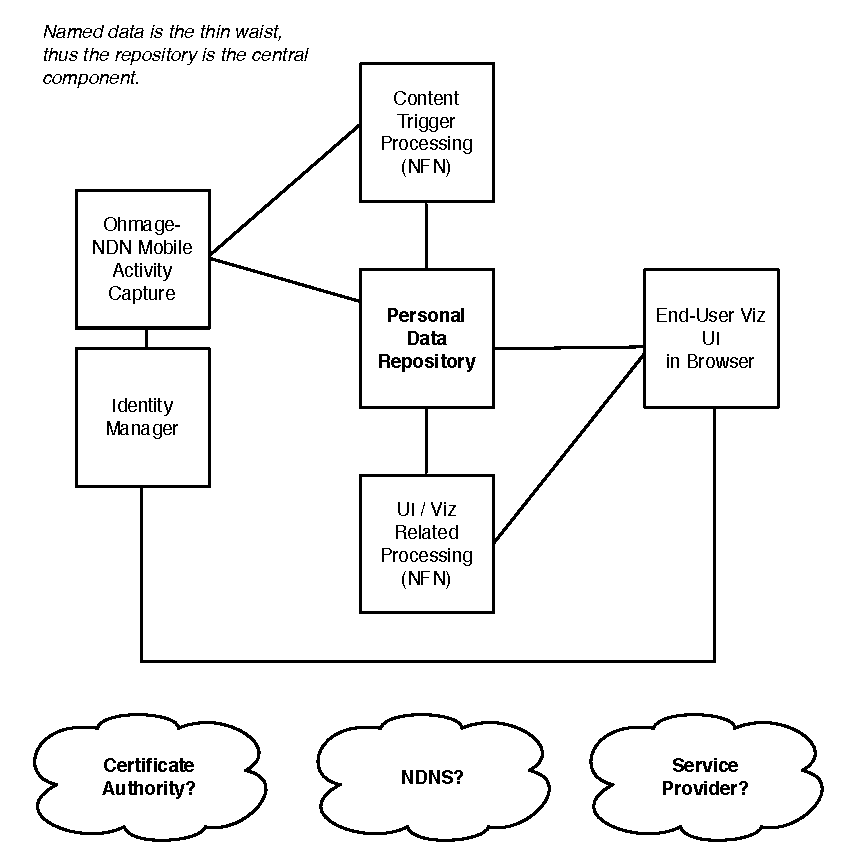
\includegraphics[width=.8\textwidth]{figures/NDNFit-App-Architecture-01}
\caption{Draft NDNFit ecosystem design.}
\label{fig:NDNFit-ecosystem}
\end{center}
\end{figure}


%%%%%%%%%%%%%%

\subsubsection{Ohmage-NDN Mobile Activity Capture}

\paragraph{Responsible team members}
Anyang University. UCLA IRL.

\paragraph{Function}
Capture location and activity information, publish. 

\paragraph{Approach}
 
Initially, we will only support Android. Port NFD, tools. Provide NDN-CCL and NFD support for Android. 

Mobile capture application is one of two primary user interfaces.  

Initial analysis of Ohmage mobile client communication completed by Prof. Euihyun Jung�s group from Anyang Univ.   

Based on the previous analysis, Prof. Euihyun Jung�s group and UCLA IRL have built a running NDNFit Android data capture application. This application captures time-location data and produce Data and temporarily stored these Data locally; when there is network connection, the NDNFit application will automatically upload Data to the DSU and delete the local copy. Figure~\ref{fig:NDNFit-UI} shows the UI of NDNFit data capture application. To use it, users only need to click ``Start Tracking�� and ``Stop Tracking��, all the other steps will be completed automatically by the application.

\begin{figure}
\begin{center}
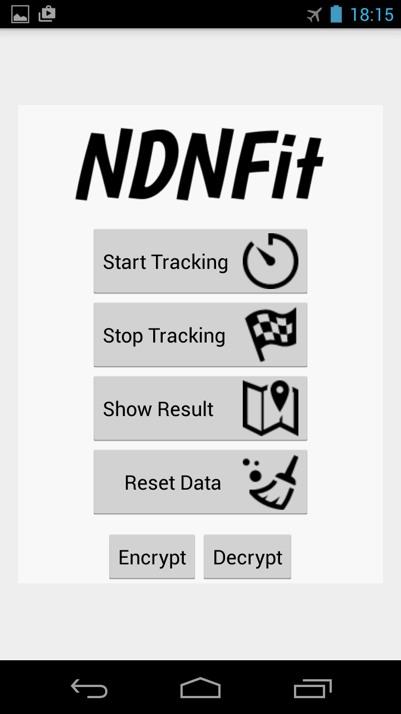
\includegraphics[width=0.4\textwidth]{figures/NDNFit.png}
\caption{NDNFit Application UI}
\label{fig:NDNFit-UI}
\end{center}
\end{figure}

From Basel: Today, we had an internal presentation from the Psychology Dept which explained their use of the Ohmage system that is running in Basel. Although NDNFit comes too late for being applied in ongoing projects, these projects are a good source of insights about user requirements for our future NDNFit system, especially the aspect of data sovereignty.

\paragraph{Building Block: Ohmage \& Mobility}

\url{http://ohmage.org/}
We are going to use the Ohmage Android client (including the Mobility module) with only the in-app storage and communication changed to NDN. See (Tangmunarunkit, H., et al., 2014) and also the papers on the Ohmage website. Note that Mobility generates activity classified data that may not require the Activity Classification DPU in the initial version.

ohmage is an open-source participatory sensing technology platform. It supports: 1) expressive project authoring; 2) mobile phone-based data capture through both inquiry-based surveys and automated data capture as well as temporally and/or spatially triggered reminders, 3) data visualization and real-time feedback; privacy respecting data management; and 4) extensible data exploration. 

Tangmunarunkit, H., et al. "Ohmage: A General and Extensible End-to-End Participatory Sensing Platform,� ACM Trans. on Intelligent Systems and Technology (in submission), UCLA CS Technical Report 140015. (Used in 20 projects.)  \url{http://web.ohmage.org/~hongsudt/pub/ohmage_ucla_140015.pdf}

%%%%%%%%%%%%%%

\subsubsection{Personal Data Repository}

\paragraph{Responsible team members}
Design led by Jianxun in Dan Pei�s group at Tsinghua.

\paragraph{Function}

Provide Open mHealth Data Storage Unit (DSU) functionality.  (Also, ``personal data vault''.) 
Personal in that it is controlled by the end user.  NOT necessarily a home repository.  More realistically, a storage service with fiduciary responsibility to protect the data of the end-user per Kang et al. 

\paragraph{Approach}

One or more new NDN repo designs supporting a hierarchy of storage needs: mobile device, user private repository, temporary processing storage.
Storage at:
\begin{itemize}
\item The mobile device itself.
\item A personal data repository (which may be distributed).
\item Temporary storage for processing and visualization components. 
\end{itemize}

Current plan:  implement in Java using jNDN, for Android support.  

\paragraph{Reference: Open mHealth Data Storage Unit (DSU) Design}

\url{https://github.com/openmhealth/developer/wiki/DSU-Overview}

The Open mHealth DSU (Data Storage Unit) API Specification is an open specification for unified information sharing across disparate data streams. The idea is simple: create an easy-to-understand set of APIs that allow siloed data stores to share information. Third-party applications that understand this API specification can then create a single set of tools to access data across any of the servers.

\paragraph{Building Block: Personal Data Vault}
Reference Derek's work here? 

Mun, Min, et al. "Personal data vaults: a locus of control for personal data streams." Proceedings of the 6th International Conference. ACM, 2010.http://remap.ucla.edu/jburke/publications/Mun-et-al-2010-Personal-Data-Vaults.pdf

Kang, J., Shilton, K., Estrin, D., Burke, J. "Self-surveillance privacy." Iowa L. Rev. 97 (2011): 809.http://escholarship.org/uc/item/1jk8b2q1.pdf


%%%%%%%%%%%%%%

\subsubsection{Distributed Processing Blocks}

\paragraph{Responsible team members}
Basel

\paragraph{Function}
Goal here is to have a few representative components implemented using NFN-style approach, not exactly the processing blocks listed above, necessarily.   Start with GeoFencing, as activity classification is currently handled in the Mobility portion of Ohmage.  But, could also consider other application-specific processing ideas. 

Initially, focusing on location-based triggers (geofencing) - to trigger location-based content.

\paragraph{Approach}

Ideally, provide composable data flow inspired by Google Cloud Dataflow, Apache Spark, etc.  

Web-based front end using NDN-JS with access to geofenced location information, providing location-specific content back to the mobile user.

Related to vehicular networking work. 

\paragraph{Reference: Open mHealth Data Processing Unit (DPU) Design}

\url{https://github.com/openmhealth/developer/wiki/Open-mHealth-and-Data-Processing}

DPUs are stateless modules that input and output data. They are designed to be embedded in other software or called remotely. They do not produce anything directly visible, but are the brains and muscles of an application. The concept of a DPU is inspired by the Unix Philosophy of creating small functional tools that can be chained and reused, rather than a single large application.

\paragraph{Building Block: Named Function Networking }

\url{http://www.named-function.net/}

Names serve to access and invoke functions, which incidentally can produce passive content once it is needed. New questions arise from this point of view, namely how the network organizes the flow of functions, which brings us squarely into active networking turf. 

\paragraph{Content Source: Trails Database}

\url{http://archinect.com/news/article/111897927/tour-los-angeles-history-with-ucla-s-new-interactive-urban-trail-app}

The LASHP Trails Mobile Website gives residents and visitors to Northeast Downtown Los Angeles site-specific access to a dynamic combination of historic information and health-related activities along urban trails starting and ending at the Los Angeles State Historic Park. 

%%%%%%%%%%%%%%

\subsubsection{Visualization Interface}

\paragraph{Responsible team members}
UCLA REMAP

\paragraph{Function}
Provide basic visualization of fitness data.

\paragraph{Approach}
Start with Ohmage web front end
NDN-JS and D3
Web-based front end using NDN-JS with access to geofenced location information, providing (for example) running trail visualization.
Perhaps use many GPX format visualizers.  E.g., \url{http://flowingdata.com/2014/02/05/where-people-run/}

\paragraph{Reference: Lifestreams Dashboard}
\cite{hsieh2013acm}

\paragraph{Building Block: Analytics / Presentation: Ohmage Front-end for Mobilize}

\url{https://wiki.mobilizingcs.org/app/web}

And Lifestreams?
Web-based front end using NDN-JS to access derived data without location information.
Examples: http://quantifiedself.com/fitbit/   

The web frontend (powered by the ohmage project) is used to provide students secure access to their data. It supports secure login, campaign management, data management and basic campaign monitoring and visualization. The students can review and share their data to the growing data set collected by their class. The web frontend can also be used to discover the answers to basic statistical inferences in real-time as data is being collected. When data collection is complete, the web frontend allows for easy exporting of the data to a more thorough statistical analysis tool. 



%%%%%%%%%%%%%%

\subsubsection{Identity Manager}
    
\paragraph{Responsible team members}
UCLA IRL (Yingdi)? and REMAP (Dustin)?
  
%%%%%%%%%%%%%%%%%%%
  
\subsection{Naming}

\paragraph{Responsible team members}
UCLA REMAP, UCLA IRL


\subsubsection{Data}
Personal health data (and metadata) namespace and repository design � focusing on support for physical activity data in the first round.  
What schema? 

\textbf{Basis of design}: Open mHealth Physical Activity data schema\footnote{\url{http://www.openmhealth.org/developers/schemas/#physical-activity} and \url{http://bioportal.bioontology.org/ontologies/SNOMEDCT?p=classes&conceptid=68130003}}, as well as other schemas from Open mHealth as needed. 

\begin{listing}
\begin{minted}[frame=single,
               framesep=3mm,
               linenos=false,
               fontsize=\footnotesize,
               tabsize=2]{js}
{     
    "$schema": "http://json-schema.org/draft-04/schema#",

    "description": "This schema represents a single episode of physical activity.",
    "type": "object",
    "references": [
        {
            "description": "The SNOMED code represents Physical activity (observable entity)",
            "url": "http://purl.bioontology.org/ontology/SNOMEDCT/68130003"
        }
    ],
    "definitions": {
        "activity_name": {
            "$ref": "activity-name-1.0.json"
        },
        "length_unit_value": {
            "$ref": "../generic/length-unit-value-1.0.json"
        },
        "time_frame": {
            "$ref": "../generic/time-frame-1.0.json"
        }
    },

    "properties": {
        "activity_name": {
            "$ref": "#/definitions/activity_name"
        },
        "effective_time_frame": {
            "$ref": "#/definitions/time_frame"
        },
        "distance": {
            "description": "The distance covered, if applicable.",
            "$ref": "#/definitions/length_unit_value"
        },
        "reported_activity_intensity": {
            "description": "Self-reported intensity of the activity performed.",
            "type": "string",
            "enum": ["light", "moderate", "vigorous"]
        }
    },

    "required": ["activity_name"]
}
\end{minted}
\caption{Open mHealth Physical Activity Schema, retrieved December 28, 2014. See appendix for subschema.} 
\label{listing:physical-activity-json}
\end{listing}




The proposed data namespace is shown in Figure~\ref{fig:NDNFit-namespace}. Its components are discussed briefly here (The black part is what we have reached agreement on, and the gray part is what needs more discussions and feedbacks):

\begin{itemize}
\item Trust anchor

The root \url{/org/openmhealth} is the trust anchor of NDNFit, users get identities and certificates from the trust anchor. 

\item DPU and DVU

NDNFit-provided DPU and DVU have identities of the format \url{/org/openmhealth/<service-id>}, they get identities and certificates from the trust anchor. Notice that non-NDNFit-provided DPU and DVU can have identities of other format, such as \url{/edu/ucla/cs/irl/speed-caculator}, \url{/edu/ucla/remap/distance-caculator} and so on.

\item User's data

Each user has an identity \url{/org/openmhealth/<user-id>}. Users get identities and certificates from the trust anchor.

A user can possess multiple mobile devices, to differentiate them, the user can further assign identity \url{/org/openmhealth/<user-id>/<device-id>} and issue certificate to each of them.

\begin{itemize}
	\item Data - data branch
	
	The original Data has 3 levels of types. In the example (so the first implementation), they are \url{fitness}(first level), \url{physical_activity}(second level) and \url{time_location}(third level). Under \url{time_location node}, there are 3 branches. The leftmost branch stands for captured data. Each data packet can have multiple samples (time location points) in it, in which case the timestamp component in its name is the start timestamp of all the samples. The middle branch is catalog. Catalogs are generated every 10 minutes (or other more appropriate time interval), the timestamp components in their names must be \url{YYYY-MM-DDTHH:MM:00Z}. Each catalog data packet contains all the names of captured data whose timestamp falls into the time span (this catalog's timestamp ~ next catalog's timestamp). The rightmost branch is C-KEY which is used for data access control, we will discuss this in data access control section.
	
	The DPU-processed data are published in the bout branch. Similar to the original data branch, the leftmost branch stands for processed data, the middle branch stands for catalog, and the rightmost branch is C-KEY.
	
	\item Data access control - read branch
	
	Name-based access control is used here. Take captured data as an example to illustrate how it works here in NDNFit.
	
	Every hour, a new C-KEY (symmetric key) is generated and used to encrypt all the captured data in this hour. The C-KEY is encrypted by the E-KEY of each access group who has access to the corresponding captured data, and is named \url{/<prefix>/C-KEY/<start_timestamp_hour>/<end_timestamp_hour>/<E-KEY name>}. The \url{start_timestamp_hour} and \url{end_timestamp_hour} are the start and end hour points when the C-KEY is valid. For each access group, the E-KEY and D-KEY (asymmetric key pair) are also generated periodically (the period is not fixed to 1 hour). The E-KEY is named
	\url{/<prefix>/E-KEY/<start_timestamp_hour>/<end_timestamp_hour>/}; and the D-KEY is encrypted for each member (data consumer) of this access group and named \url{/<prefix>/D-KEY/<start_timestamp_hour>/<end_timestamp_hour>/for/<consumer-id>}. Notice that in this case, all the C-KEYs, E-KEYs and D-KEYs are generated by the user.
	
	For the DPU-processed data (the bout branch), it's a little complicated. In this case, the C-KEY should be generated by the DPU, and then it should be sent back to the user (the C-KEY should be encrypted only for the user) to be encrypted by some access groups? E-KEYs. All the other steps are the same as the previous.
	
	\item Data publish control - write branch
	
	When a DPU processes user's data, it should use some valid signing key to sign the processed results. The signing key pair is generated by the DPU, the private key is kept by the DPU and the public key is sent back to the user. Then the user checks whether the public key is named properly (so data consumers can validate the signature of processed results according to trust schema), if it is, the user can sign and publish this public key. The name structure of this public key is similar to that of D-KEYs.
	

\end{itemize}
\item User group
	
Some users can form groups. Groups have identities of the format \url{/org/openmhealth/<group-id>}. This is not part of first implementation. Details will be discussed in the future.

\end{itemize}


\begin{figure}
\begin{center}
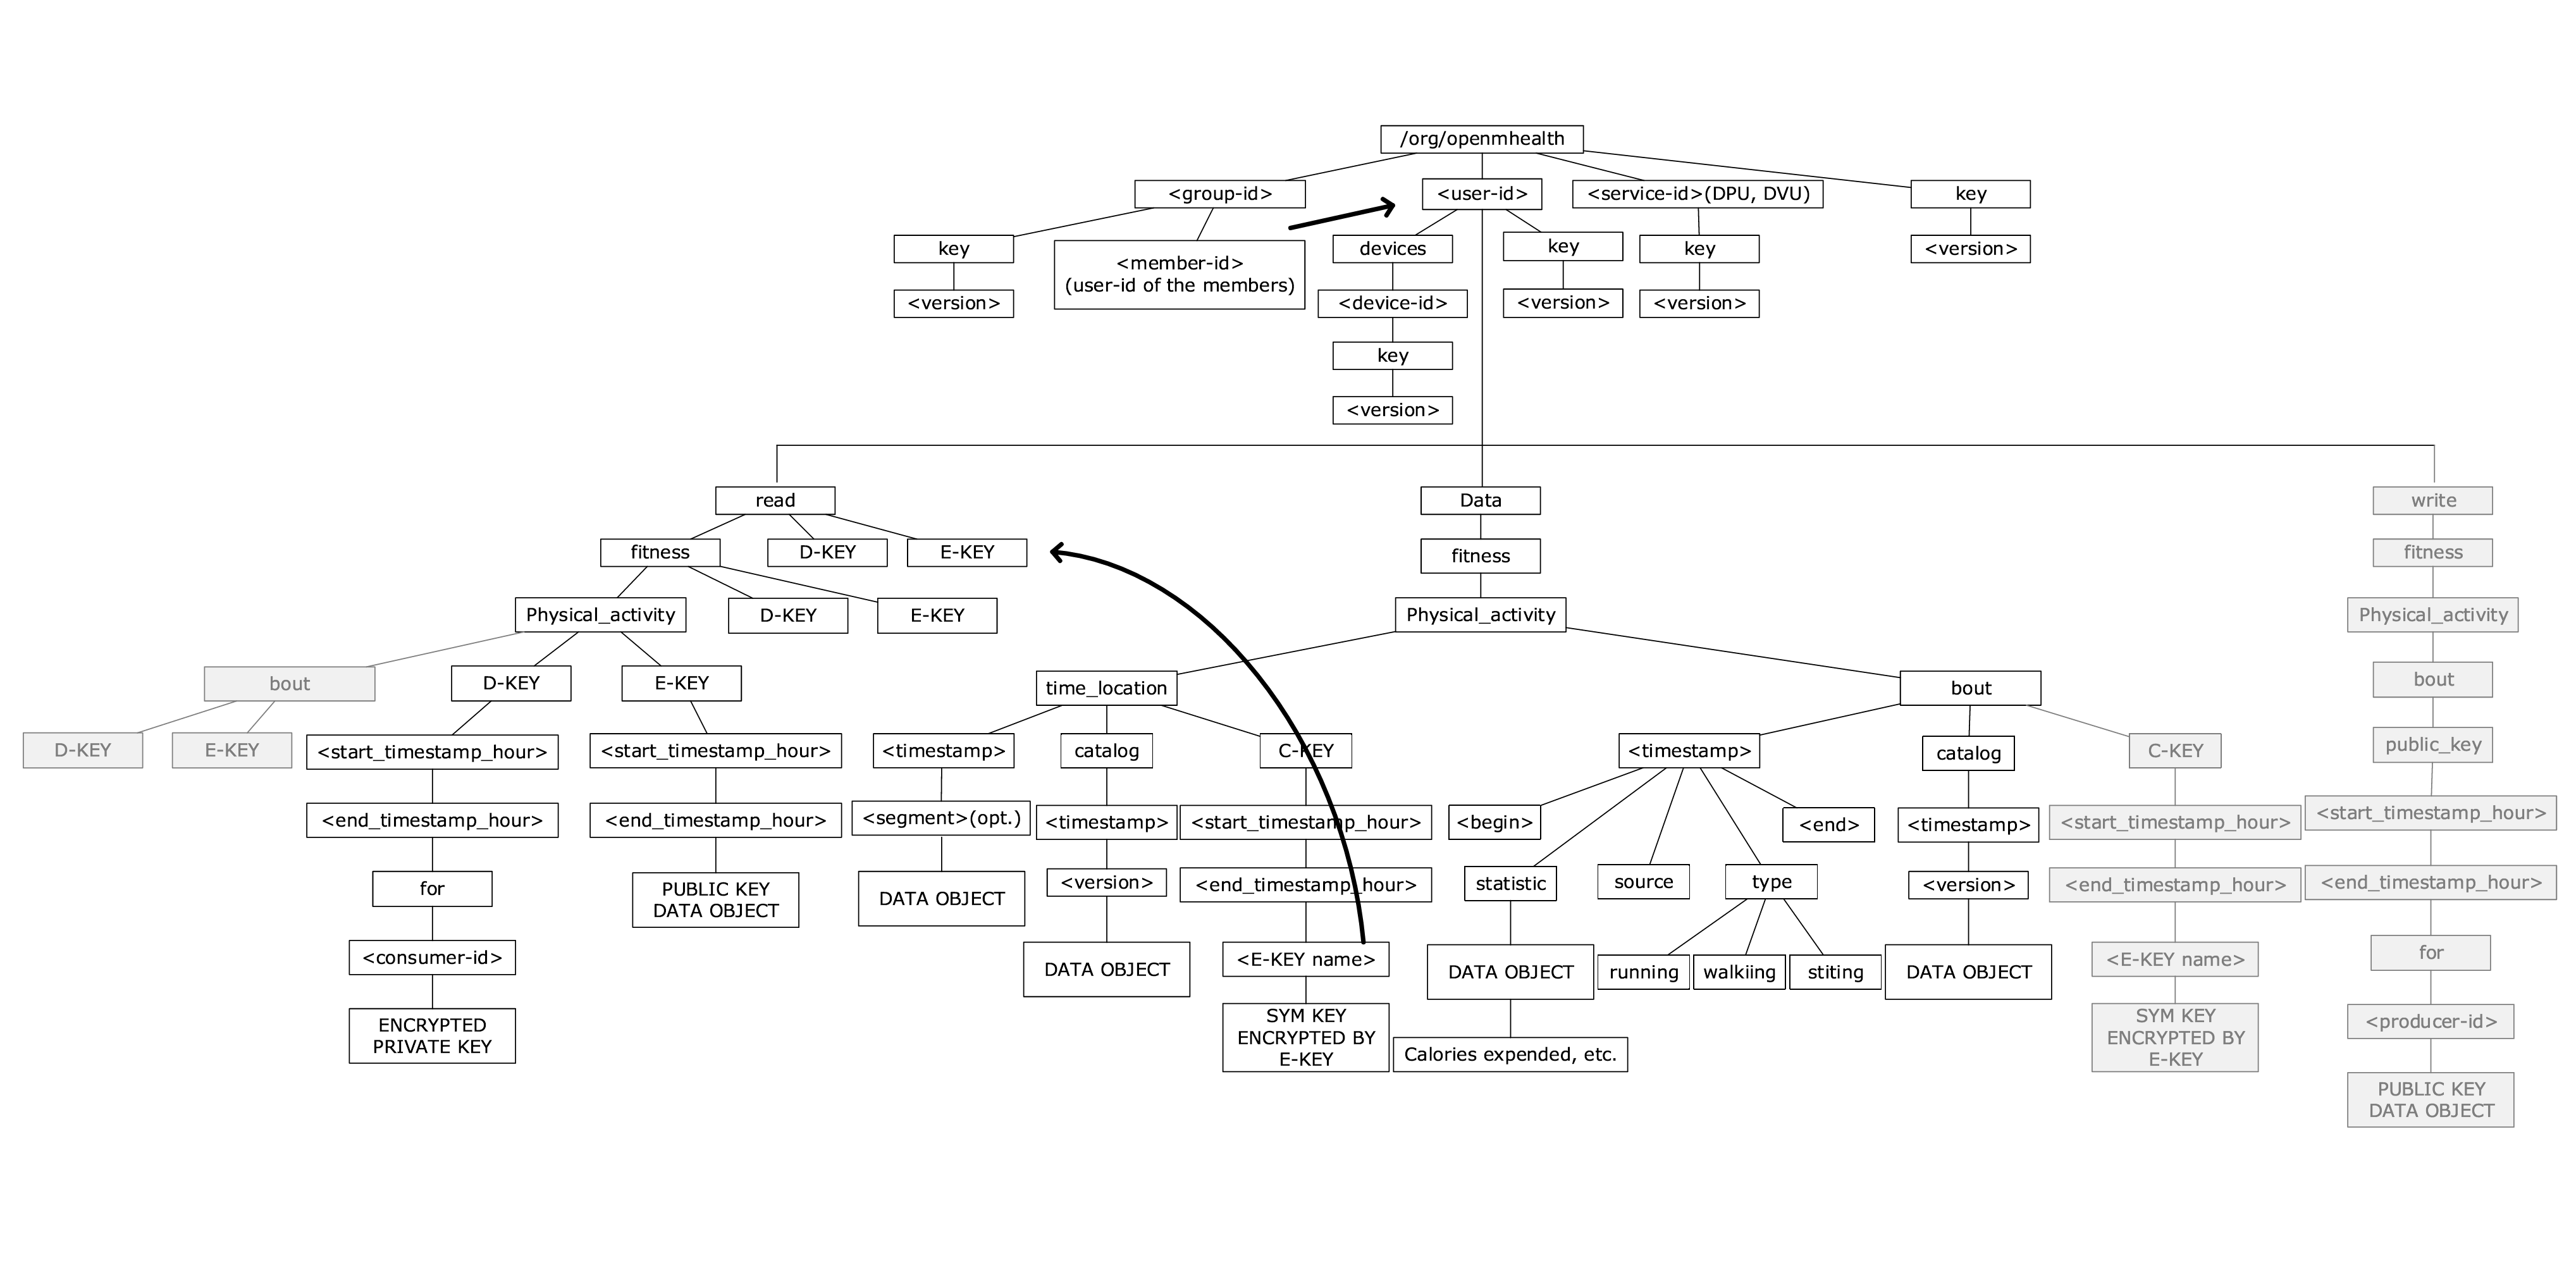
\includegraphics[width=0.65\textwidth]{figures/NDNFit-name-top-02.png}
\caption{NDNFit Namespace, version 2.}
\label{fig:NDNFit-namespace}
\end{center}
\end{figure}

\subsubsection{Certificates}

\subsubsection{Processing}
Borrow ideas from Named Function Networking concept for distributed processing

%%%%%%%%%%%%%%
  
\subsection{Trust and security}

\paragraph{Responsible team members}
U. Michigan, UCLA IRL, UCLA REMAP

\subsubsection{Trust model} 

In this application, the user should be the root of trust for their own data, though this may be enabled
by various service providers. 

If possible, we would like to leverage the existing PKI/SPKI support in NDN, and take advantage of the
existing infrastructure.  \emph{However}, certificates used should not leak real world identity 
information except by the choice of the user. 

One entity (here, the `` user") maintains multiple publishers whose data are
consumed by many services with varying levels of access based on the: type
of data (as expressed in the name), level of granularity, and date/time
when the data was produced. ABE seems a good fit here, is it viable for
practical experimentation or do we need a directory-of-symmetric-keys or
some other approach?  If not ABE, where should we begin for our approach?
Are there existing best practices?

\subsubsection{Identity}

% Commenting out the old text for identity

% Users may have different identities per service (or at least per flow). 

% We are exploring the idea of an ``identity manager", an application
% manages the certificates (identities) that an individual uses to interact
% with the various services involved in this application. Are there good
% examples of \emph{user interfaces} for identity management already?  In fact,
% pointers to state-of-the-art in end-user interfaces for security decision
% making would be helpful. Alex doesn't think there are many. 

% Each step in the data processing model tends to generate derived data that must also be stored and 
% may or may not be associated with the original identity.  

Three types of identities are involved in the NDNFit application. A user identity, which associates with a user of applications in the Open mHealth ecosystem; a device identity, which associates with a device that the user owns; and an application identity, which associates with an application installed on a device.

User and device identity generation are handled by a separate application called ``identity manager'' (ID manager). In the case of NDNFit, to generate a user identity, the ID manager first asks the Open mHealth authority for a namespace under which its data can be published, then generates a key for that namespace, and asks the Open mHealth root of trust to sign that key and provide a certificate. The interaction between ID manager and Open mHealth root of trust goes through email and http requests: that is, the Open mHealth authority will associate an assigned namespace with a user that owns the email address he provided. Device identity is generated by the identity manager, and signed by the user identity. User identities may be used to sign device identities for each device that the user owns, but the first iteration of the design does not cover this interaction.

An application identity is generated upon the first launch of the application. The application asks the ID manager on the same device for the data publishing namespace, and generates a key for that data namespace. This key is signed by the device identity, and is used to sign the data produced by the application.

For a user's data to be verified, application certificates, device certificates, and user certificates need to be published.

An example of the trust relationship is given in Figure \ref{fig:identity}.

\begin{figure}
\begin{center}
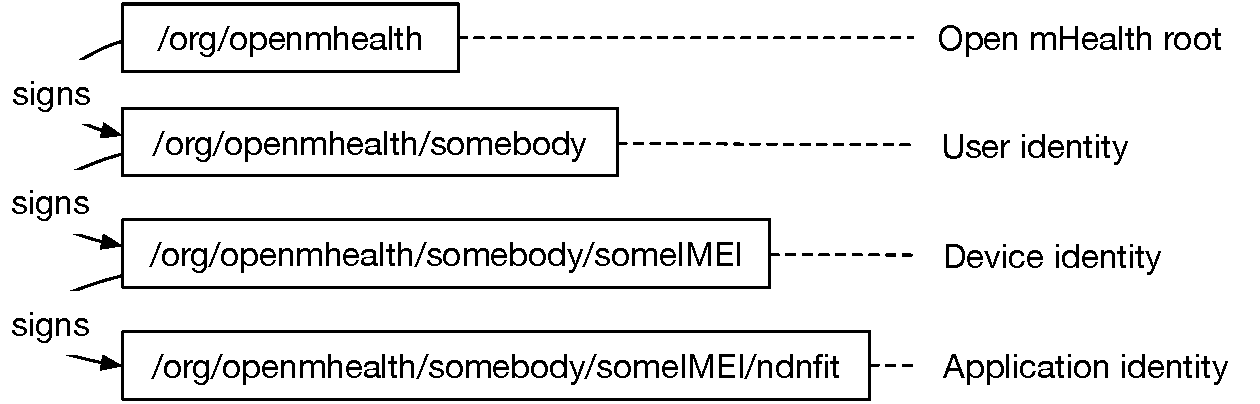
\includegraphics[width=0.75\textwidth]{figures/NDNFit-identity-example}
\caption{User, device, and app identity for NDNFit application}
\label{fig:identity}
\end{center}
\end{figure}

\subsubsection{Integrity} 

\subsubsection{Confidentiality}

Principal of minimum information:  services should only request / consume the minimum 
amount of information needed to complete their application. 

We will need to come up with an approach for name encryption for
this environment, in a way that still enables applications to operate on
the namespace--perhaps without having to be concerned with
decryption--once it has been decrypted and/or de-encapsulated.

Public access should be considered but is primarily for future access. 
Extensions to support epidemiological studies incorporating semi-anonymized opt-in data across large populations. 


\subsubsection{Data flow model support}

Must consider access control for services 
in "data flow" model for communication between processing components, replacing Oauth. 

We imagine a data flow like model for this system:
[Publisher]->[Processing]->[Processing]->[Visualization], with each []
block being owned by a different entity and an objective to leak the
minimum amount of context to the processing components.  I'm not sure we
understand how to handle authentication /  access control of the
intermediate processing blocks, to each other and to the source/sink of
the data.  Where can we look for best practices for security in current
data flow architectures?

%%%%%%%%%%%%%%

%%%%%%%%%%%%%%
  
\subsection{Storage}

\paragraph{Responsible team members}
UCLA IRL, Tsinghua, UCLA REMAP

A distributed network of repos replaces the ecosystem of DSUs envisioned in the Open mHealth TCP/IP architecture. 

(Hierarchical network of repositories, similar to BAS/BMS, including both personal repositories, service provider backups for personal data, and aggregated "anonymized" stores). 

Need to provide write access control

A mechanism for delegating authority to publish into a repository is
necessary. 

%%%%%%%%%%%%%%
  
\subsection{Routing \& Forwarding}

\paragraph{Responsible team members}
UCLA IRL

Mobile publishing support. NDNS?

\begin{figure}
\centering
\subfigure[Mobile publisher connected to ``home'' hub, which directly routes its publishing prefix.]{
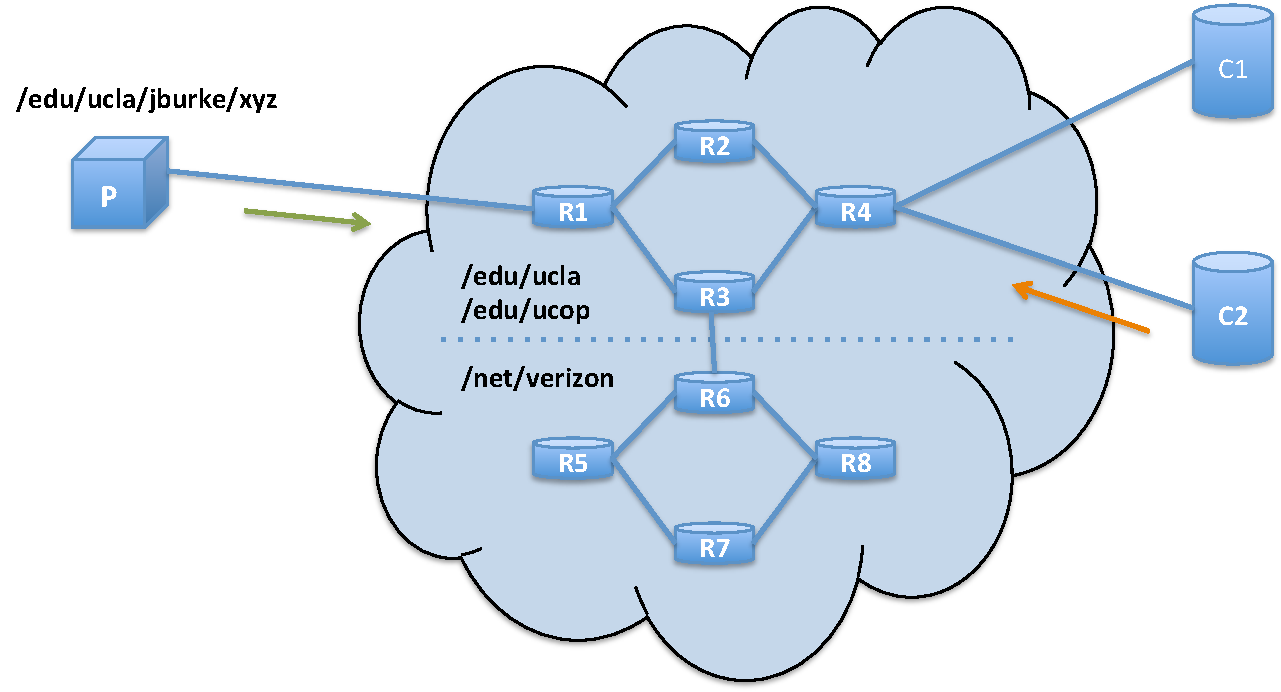
\includegraphics[width=0.45\columnwidth, keepaspectratio=true]{figures/publisher-mobility-a}
}
\subfigure[Mobile publisher connected to another hub, which does not directly route its prefix.]{
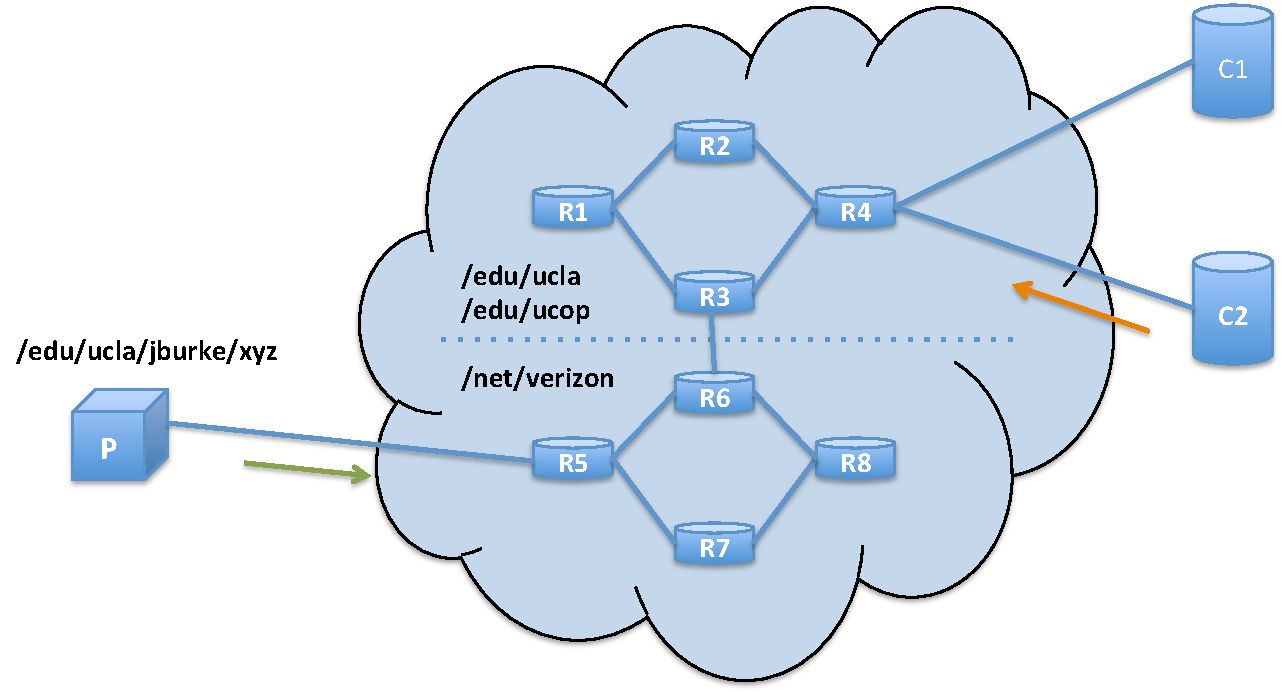
\includegraphics[width=0.45\columnwidth, keepaspectratio=true]{figures/publisher-mobility-b}
}
\caption{Mobile publisher scenario.}
\label{fig:mobilepublisher}
\end{figure}


